\section{Interferometric Diagnostics and the Abel Transform}

The propagation code produces a three dimensional map of the free electron density, the self-trapped exciton density, and the intensity, but none of these quantities can be measured directly inside a bulk sample. What can be measured is the phase shift accumulated by a probe beam that crosses the excited region, using a Nomarski interferometer. This section derives how that phase shift relates to the refractive index change predicted by the simulation, and describes how the program implements it.

\subsection{Two-Plane-Wave Interferometry}

The Nomarski interferometer can be understood as a configuration that allows retrieval of phase information about a medium under investigation. We derive the fundamental equations governing the interference pattern produced by two plane waves with different propagation directions.

\subsubsection{Electric Fields and Wave Vectors}

Consider two plane waves propagating in the same medium with refractive index $\eta_i$:
\begin{equation}
E_1 = \underline{E_0} \, e^{i(\vec{k}_1 \cdot \vec{r} - \omega t)}
\end{equation}
\begin{equation}
E_2 = \underline{E_0} \, e^{i(\vec{k}_2 \cdot \vec{r} - \omega t)}
\end{equation}
where the wave vectors are defined as:
\begin{equation}
\vec{k}_1 = \frac{2\pi}{\lambda}\eta_i \begin{pmatrix}\sin{\theta}\\0\\\cos{\theta}\end{pmatrix} = k \begin{pmatrix}\sin{\theta}\\0\\\cos{\theta}\end{pmatrix}, \qquad
\vec{k}_2 = k \begin{pmatrix}-\sin{\theta}\\0\\\cos{\theta}\end{pmatrix}
\end{equation}
These two plane waves propagate symmetrically with respect to the normal axis, making an angle $2\theta$ with each other. To account for an arbitrary orientation of the fringes around the $z$ axis, we introduce a rotation of angle $\phi$, which turns the wave vectors into $k(\cos\phi\sin\theta,\sin\phi\sin\theta,\cos\theta)$ and its mirror image.

\subsubsection{Intensity Distribution and Fringe Spacing}

Setting the observation screen at $z=0$, the intensity is:
\begin{equation}
I(x,y) = I_1 + I_2 + \sqrt{I_1I_2} \cos\big((\vec{k}_1 - \vec{k}_2) \cdot \vec{r}\big)
\end{equation}
For equal amplitudes and after computing the phase difference $(\vec{k}_1-\vec{k}_2)\cdot\vec{r} = 2k\sin\theta(x\cos\phi+y\sin\phi)$, this becomes:
\begin{equation}
\boxed{I(x,y) = 2I_0(x,y)\left[1 + \cos\big(2\pi \nu_0(x\cos{\phi}+y\sin{\phi}\big)\right]}, \qquad \nu_0 = \frac{2\sin\theta}{\lambda}
\label{eq:carrier_freq}
\end{equation}
where $\nu_0$ is the spatial-carrier frequency of the fringes, set purely by the crossing angle $2\theta$ of the two interfering beams, and independent of anything happening inside the medium.

\begin{figure}[h!]
    \centering
    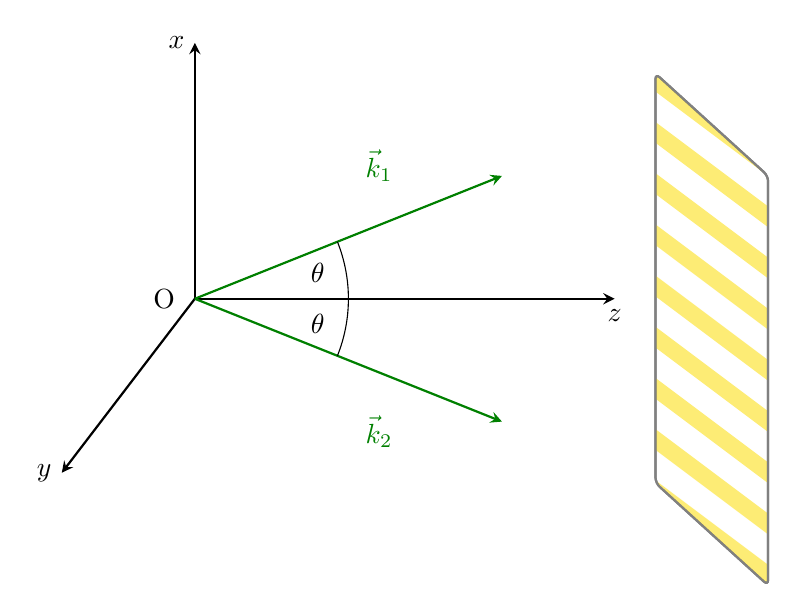
\begin{tikzpicture}[scale=1.3]
        \draw[-stealth, thick] (0,0) -- (0,2.5) node[left] {$x$};
        \draw[-stealth, thick] (0,0) -- (-1.3,-1.7) node[left] {$y$};
        \draw[-stealth, thick] (0,0) -- (4.1,0) node[below] {$z$};
        \node[left] at (-0.1, 0) {O};
        \def\screen{
            (4.5, 2.2) -- (5.6, 1.2) -- (5.6, -2.8) -- (4.5, -1.8) -- cycle
        }
        \draw[gray, thick, fill=white, rounded corners=2pt] \screen;
        \begin{scope}
            \clip[rounded corners=2pt] \screen;
            \foreach \i in {-4,-3.5,...,4} {
                \draw[yellow!80!orange, line width=6pt, opacity=0.55] (4, \i) -- (6, \i-1.5);
            }
        \end{scope}
        \draw[gray, thick, rounded corners=2pt] \screen;
        \draw[-stealth, thick, green!50!black] (0,0) -- (3, 1.2);
        \node[green!50!black] at (1.8, 1.3) {$\vec{k}_1$};
        \draw[-stealth, thick, green!50!black] (0,0) -- (3, -1.2);
        \node[green!50!black] at (1.8, -1.3) {$\vec{k}_2$};
        \draw (1.5,0) arc (0:21.8:1.5);
        \node at (1.2, 0.25) {$\theta$};
        \draw (1.5,0) arc (0:-21.8:1.5);
        \node at (1.2, -0.25) {$\theta$};
    \end{tikzpicture}
    \caption{Interference of two plane waves propagating symmetrically with an angle $2\theta$, creating an interference pattern on the screen (shown for $\phi = 0$).}
    \label{fig:interference}
\end{figure}

\subsection{Phase and Amplitude Extraction via Fourier Analysis}

Nomarski interferograms read $I(x,y) = a(x,y) + b(x,y)\cos\!\big[2\pi\nu_0 x + \varphi(x,y)\big]$, where $a(x,y)$ is the background term, $b(x,y)$ the amplitude modulation term, and $\varphi(x,y)$ the phase of interest, related to the line integrated electron density by $\varphi(x,y) \propto \int n_e(x,y,z)\,\mathrm{d}z$. In conventional contour-fringe interferometry, obtained when $\nu_0=0$, the intensity reads $I = a + b\cos\varphi$, in which $a$, $b$, and $\varphi$ are mixed, which limits accuracy, and the parity of the cosine prevents determining the sign of $\varphi$.

The Takeda method~\cite{takeda1982fourier} overcomes both limitations through spatial heterodyne demodulation. As in classical heterodyne detection, the signal of interest is carried by an oscillating reference, here the spatial carrier $\nu_0$ generated by the tilted incidence angle of the interferometer arms. Writing the cosine with Euler's formula gives $I(x,y) = a(x,y) + c(x,y)e^{i2\pi\nu_0 x} + c^*(x,y)e^{-i2\pi\nu_0 x}$ with $c(x,y) = \tfrac{1}{2}b(x,y)e^{i\varphi(x,y)}$. Bandpass filtering around $+\nu_0$ in the Fourier plane isolates the sideband carrying $c(x,y)$ alone, from which $b$ and $\varphi$ are recovered respectively as the modulus and the argument.

This linear separation also improves sensitivity to weak phase variations. Contour interferometry responds quadratically to a small phase, $\Delta I_{contour} \approx \tfrac{b}{2}\varphi^2$, because small variations sit near the extremum of a cosine, whereas the Takeda method responds linearly, $\Delta I_{Takeda} \approx -b\sin(2\pi\nu_0 x)\,\varphi$, which is what gives it sub-wavelength phase sensitivity~\cite{takeda1982fourier}. Applied to a reference interferogram (no plasma or no excitation) and a measurement interferogram, the ratio of the two filtered and inverse transformed signals cancels the carrier and any residual optical misalignment:
\begin{equation}
z(x,y) \equiv \frac{I_{\text{meas,filt}}(x,y)}{I_{\text{ref,filt}}(x,y)} = \frac{b_2(x,y)}{b_1(x,y)}\,e^{i\varphi(x,y)}, \qquad
\boxed{\varphi(x,y) = \operatorname{atan2}\big(\Im{(z)},\Re{(z)}\big)}
\end{equation}

\subsection{Resolution Limits}

Two independent limits set the finest feature that can be resolved. The Nyquist limit comes from the pixelated sensor. The shortest oscillation observable without aliasing must span at least two pixels, giving $\nu_N = 1/(2\Delta x)$ with $\Delta x$ the pixel size. The optical limit comes from diffraction at the sample itself. A feature of size $d$ diffracts light at an angle $\sin\theta = \lambda/d$, and this diffracted light is only collected by the imaging lens if $\sin\theta \le NA$.

\usetikzlibrary{decorations.pathmorphing, arrows.meta, angles, quotes}

\subsection{Spatial and Frequential Resolutions}
\subsubsection{Nyquist Frequency Limit}
We've seen the principles of the Takeda method to recover fine phase information by modulating spatial frequency via a Wollaston cube. However to be able to observe very fine detuning we need to use digital analysis and therefore use a camera sensor to capture the holographic interference pattern. 
This conversion from continuous to discrete signals (analogue to digital) comes with some limitations we will try to explain in this section.

The first limitation comes from the Nyquist frequency limit. On a discret sample, the shortest oscillation that can be observed without aliasing effect, has to spread on two pixels, an alternance of high and low value of the light intensity. The shortest period observed is then limited by the size of these two successive pixels. Thus the Nyquist frequency limit is defined as $$\nu_N= \frac{1\,\text{period} }{2 \, \text{pixels}}= \frac{1}{2\Delta x}\, \, \, \,  \text{with} \, \Delta x = \text{pixel size}$$
However with a 45° orientation of successive fringes, the value of successive pixels can be calculated from a continuous intensity function $\cos^2(2\pi f_x x +2\pi f_y y +\phi) $ as : 
$$I(n_x,n_y) = \int^{n_x+\frac{1}{2}}_{n_x-\frac{1}{2}}\int^{n_y+\frac{1}{2}}_{n_y-\frac{1}{2}}\cos^2(2\pi f_x x +2\pi f_y y +\phi)\, dx \,dy $$
$$ I(n_x, n_y) = \frac{1}{2} + \frac{1}{2} \cos(2\pi f_x n_x + 2\pi f_y n_y +\phi) \left[ \frac{\sin(\pi f_x)}{\pi f_x} \right] \left[ \frac{\sin(\pi f_y)}{\pi f_y} \right] $$
With $f_x = f_y = \frac{1}{2}$:
$$ I(n_x, n_y) = \frac{1}{2} + \frac{1}{2} \cos(\pi (n_x + n_y)+\phi) \left[ \frac{\sin(\pi/2)}{\pi/2} \right] \left[ \frac{\sin(\pi/2)}{\pi/2} \right] = \frac{1}{2} +\frac{2}{\pi^2}\cos{(\pi(n_x+n_y)+\phi)} $$
This function is maximum for $\phi = 0$ and pixel value alternates between two value  $$\frac{1}{2} \pm \frac{2}{\pi^2}$$
\begin{figure}[h]
    \centering
    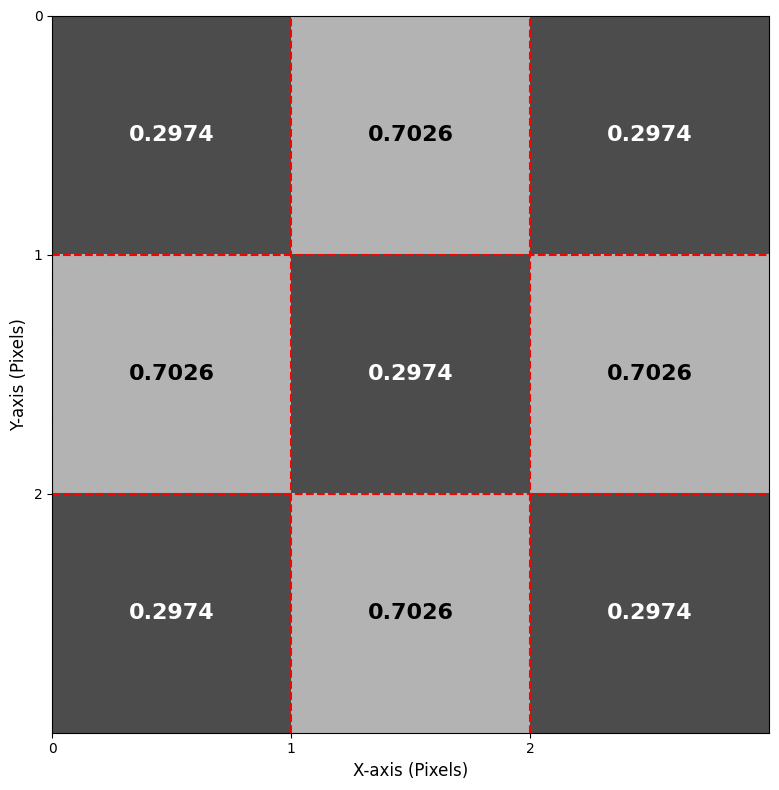
\includegraphics[width=0.41\linewidth]{pixel value.png}
    \caption{Exact Spatial Integration over Square Pixels at Nyquist Limit (45°)}
    \label{fig:pixel}
\end{figure}

\subsubsection{Sample Diffraction and Smallest Resolved Feature}
On the other hand, the highest spatial frequency transmitted by the optical system is limited by the size of the smallest feature of the sample we try to capture. 
The plasma acts as a diffracting object for incident light beams. The first order deflection angle is given by the path difference $\Delta l = d\sin{\theta}$, where $d$ is the caracteristic size of the diffracted object.
The corresponding detuning term reads : $$k\Delta l = \frac{2\pi}{\lambda}d\sin{\theta}$$
Constructive interference between contributions of successive periods of the diffracting object occurs when $k\Delta l = m2\pi$, defining the diffraction orders.
In the case of a first order diffraction $m = \pm 1$: Thus the first order diffracted beam originating from a $d$ sized feature are coming with an angle $\theta$ onto the microscop lense such that $\sin{\theta} = \frac{\lambda}{d}$.

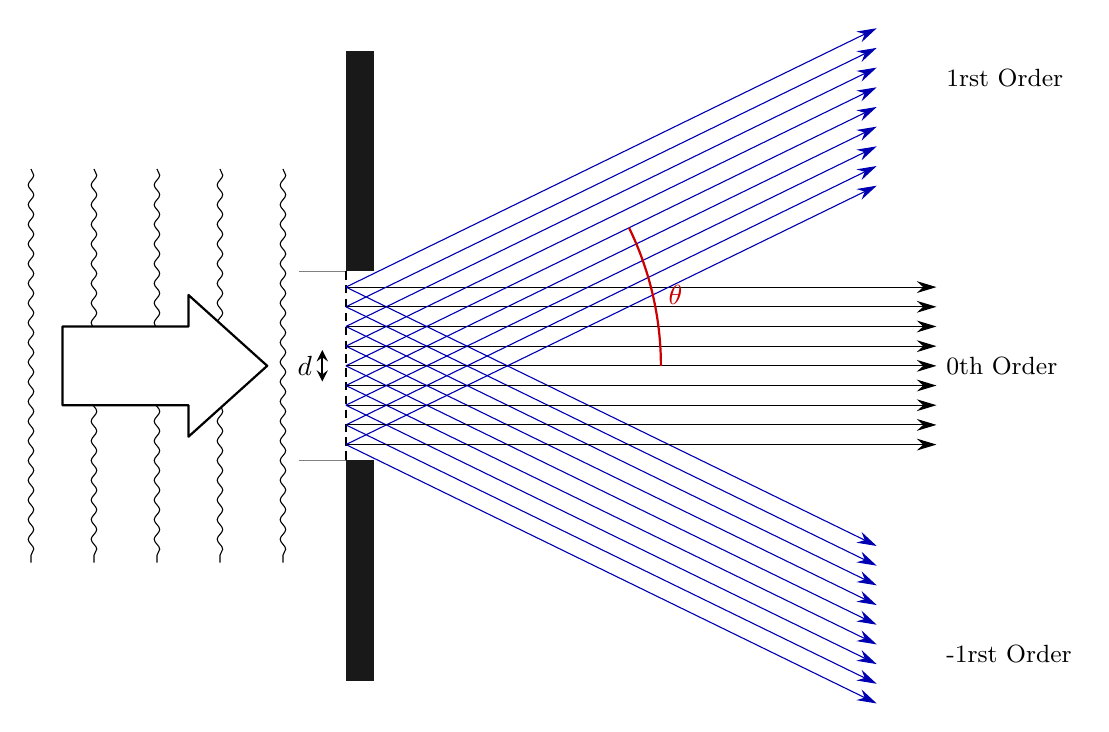
\begin{tikzpicture}

% --- ONDES INCIDENTES ---
\foreach \x in {-4, -3.2, -2.4, -1.6, -0.8} {
    \draw[decorate, decoration={snake, amplitude=0.35mm, segment length=2.5mm}, thin] (\x, 2.5) -- (\x, -2.5);
}

% Flèche de direction
\draw[thick, fill=white, line join=round] (-3.6, -0.5) -- (-2.0, -0.5) -- (-2.0, -0.9) -- (-1.0, 0) -- (-2.0, 0.9) -- (-2.0, 0.5) -- (-3.6, 0.5) -- cycle;

% --- OBSTACLE ET FENTE ---
\fill[black!90] (0, 1.2) rectangle (0.35, 4);
\fill[black!90] (0, -1.2) rectangle (0.35, -4);

% Indication de la largeur d
\draw[<->, >=stealth, thick] (-0.3, 0.2) -- (-0.3, -0.2) node[midway, left] {$d$};
\draw[thin, gray] (-0.6, 1.2) -- (0, 1.2);
\draw[thin, gray] (-0.6, -1.2) -- (0, -1.2);

% Ligne pointillée (ouverture)
\draw[densely dashed, thick] (0, 1.2) -- (0, -1.2);

% --- RAYONS DIFFRACTÉS ---
% Définition de l'angle de déviation
\def\angleDev{26} 

\foreach \y in {1.0, 0.75, 0.5, 0.25, 0, -0.25, -0.5, -0.75, -1.0} {
    % Ordre +1
    \draw[-{Stealth[length=2.5mm, width=1.5mm]}, blue!70!black, thin] (0, \y) -- ++(\angleDev:7.5);
    
    % Ordre 0 (Central)
    \draw[-{Stealth[length=2.5mm, width=1.5mm]}, black, thin] (0, \y) -- ++(0:7.5);
    
    % Ordre -1
    \draw[-{Stealth[length=2.5mm, width=1.5mm]}, blue!70!black, thin] (0, \y) -- ++(-\angleDev:7.5);
}

% --- INDICATION DE L'ANGLE THETA ---
% On définit des points pour tracer l'angle
\coordinate (A) at (0,0);
\coordinate (B) at (5,0);
\coordinate (C) at (5, {5*tan(\angleDev)});

\draw[thick, red!80!black] (4,0) arc (0:\angleDev:4) node[midway, right, xshift=2pt] {$\theta$};

% Labels des ordres
\node[right] at (7.5, {7.5*tan(\angleDev)}) {\small 1rst Order};
\node[right] at (7.5, 0) {\small 0th Order};
\node[right] at (7.5, {-7.5*tan(\angleDev)}) {\small -1rst Order};

\end{tikzpicture}


We can then invert the problem: what is the size of the smallest feature a microscope lens can resolve, knowing that the maximum acceptance angle is given by the numerical aperture? $$NA = n \sin{\alpha}\xrightarrow{n_{air}=1}\sin{\alpha}$$
For the first order diffracted beam to be collected by the lens, one must have $\sin{\theta}\leq\sin{\alpha}$, which gives the shortest resolved feature in our coherent on-axis configuration : $$R_0= \frac{\lambda}{\sin{\alpha}} = \frac{\lambda}{NA}$$
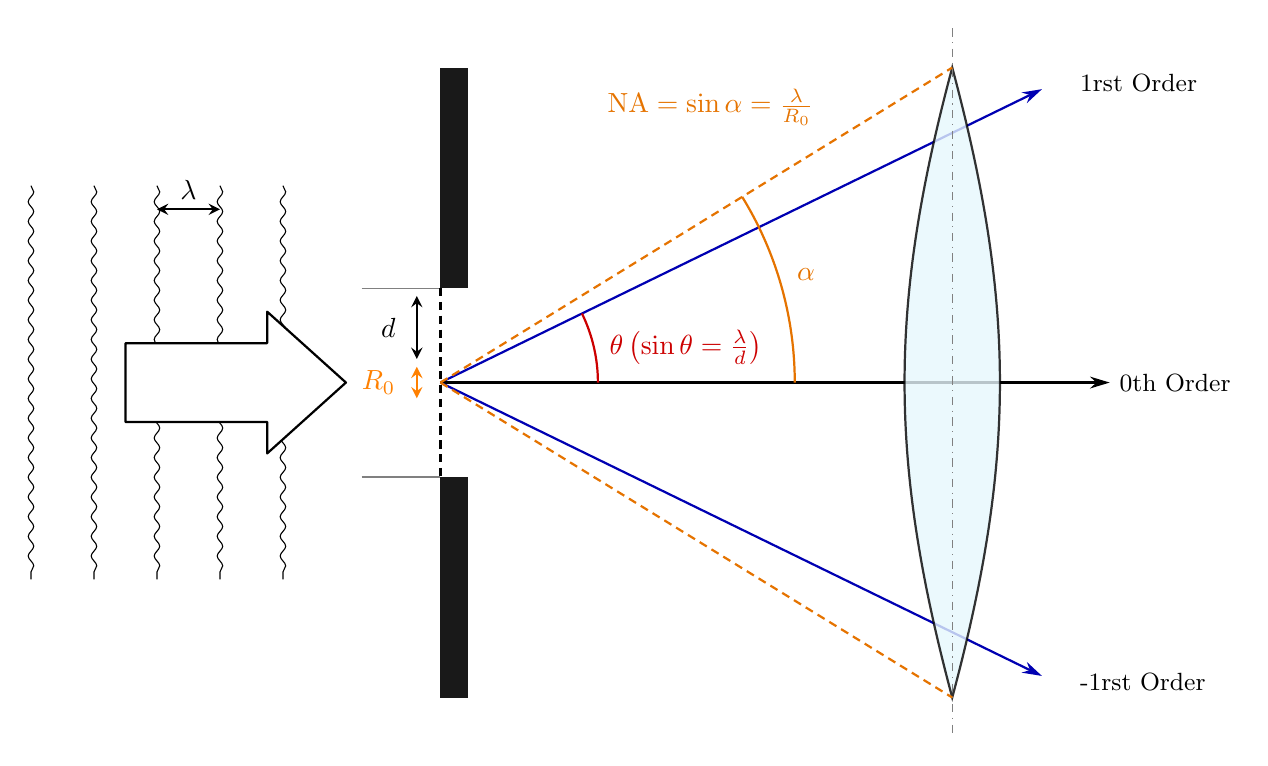
\begin{tikzpicture}

% --- ONDES INCIDENTES ---
% Décalées plus à gauche pour libérer de l'espace
\foreach \x in {-5.2, -4.4, -3.6, -2.8, -2.0} {
    \draw[decorate, decoration={snake, amplitude=0.35mm, segment length=2.5mm}, thin] (\x, 2.5) -- (\x, -2.5);
}

% Indication de la longueur d'onde \lambda
\draw[<->, >=stealth, thick] (-3.6, 2.2) -- (-2.8, 2.2) node[midway, above] {$\lambda$};

% Flèche de direction (reculée vers la gauche)
\draw[thick, fill=white, line join=round] (-4.0, -0.5) -- (-2.2, -0.5) -- (-2.2, -0.9) -- (-1.2, 0) -- (-2.2, 0.9) -- (-2.2, 0.5) -- (-4.0, 0.5) -- cycle;

% --- OBSTACLE ET FENTE ---
\fill[black!90] (0, 1.2) rectangle (0.35, 4);
\fill[black!90] (0, -1.2) rectangle (0.35, -4);

% Lignes de rappel grises (allongées pour s'adapter au texte)
\draw[thin, gray] (-1.0, 1.2) -- (0, 1.2);
\draw[thin, gray] (-1.0, -1.2) -- (0, -1.2);

% Ligne pointillée (ouverture)
\draw[densely dashed, thick] (0, 1.2) -- (0, -1.2);

% --- COTES d ET R0 ---
% Indication de la largeur d
\draw[<->, >=stealth, thick, orange] (-0.3, 0.2) -- (-0.3, -0.2) node[midway, left=4pt] {$R_0$};

% Indication de R_0 et sa formule en orange
% J'ai allongé un peu la flèche et décalé le texte (left=4pt) pour qu'il soit bien lisible
\draw[<->, >=stealth, thick] (-0.3, 1.1) -- (-0.3, 0.3) node[midway, left=4pt] {$d$};


% --- RAYONS DIFFRACTÉS ---
% Définition de l'angle de déviation
\def\angleDev{26} 

\foreach \y in {0} {
    % Ordre +1
    \draw[-{Stealth[length=2.5mm, width=1.5mm]}, blue!70!black, thick] (0, \y) -- ++(\angleDev:8.5);
    
    % Ordre 0 (Central)
    \draw[-{Stealth[length=2.5mm, width=1.5mm]}, black, thick] (0, \y) -- ++(0:8.5);
    
    % Ordre -1
    \draw[-{Stealth[length=2.5mm, width=1.5mm]}, blue!70!black, thick] (0, \y) -- ++(-\angleDev:8.5);
}

% --- LENTILLE ---
\def\lensX{6.5}
\def\lensY{4.0}
% Dessin de la lentille biconvexe
\draw[thick, fill=cyan!10, opacity=0.8] (\lensX, \lensY) to[bend left=15] (\lensX, -\lensY) to[bend left=15] cycle;
% Axe principal de la lentille
\draw[dash dot, thin, gray] (\lensX, \lensY+0.5) -- (\lensX, -\lensY-0.5);

% --- OUVERTURE NUMÉRIQUE (NA) ---
% Rayons marginaux définissant l'ouverture de la lentille
\draw[densely dashed, thick, orange!90!black] (0,0) -- (\lensX, \lensY);
\draw[densely dashed, thick, orange!90!black] (0,0) -- (\lensX, -\lensY);

% Calcul et tracé de l'angle Alpha
\pgfmathsetmacro{\angleAlpha}{atan(\lensY/\lensX)}
\draw[thick, orange!90!black] (4.5,0) arc (0:\angleAlpha:4.5) node[midway, right, xshift=2pt, yshift=4pt] {$\alpha$};

% Label NA 
\node[orange!90!black, right] at (\lensX-4.5, \lensY-0.5) {$\mathrm{NA} = \sin \alpha = \frac{\lambda}{R_0}$};

% --- INDICATION DE L'ANGLE THETA ET DE LA FORMULE ---
\draw[thick, red!80!black] (2,0) arc (0:\angleDev:2) node[midway, right, xshift=2pt] {$\theta \left( \sin\theta = \frac{\lambda}{d} \right)$};

% --- LABELS DES ORDRES ---
\node[right] at (8, {7.8*tan(\angleDev)}) {\small 1rst Order};
\node[right] at (8.5, 0) {\small 0th Order};
\node[right] at (8, {-7.8*tan(\angleDev)}) {\small -1rst Order};

\end{tikzpicture}


The more familiar Abbe formula $\tfrac{\lambda}{2NA}$ comes from tilting the illumination instead of using an axial beam. If the sample is illuminated under an angle $\alpha$, the 0th order is rejected at $-\alpha$ and a first order can still enter the lens up to $\sin\theta = 2\sin\alpha$, doubling the bandwidth. Standard microscopes reach this limit naturally with a Köhler condenser that fills the whole cone $[-\alpha,+\alpha]$. Our setup uses a coherent on-axis beam, so the resolution stays at $\tfrac{\lambda}{NA}$.


The image is then magnified via a $4f$ optical system, and thus the final smallest resolved feature visible on the sensor has a width of $R_s=M_{tot}R_0$.

In the frequency domain, the optical system acts as a low-pass filter whose cutoff is the highest spatial frequency transmitted to the sensor : $$\nu_{max} = \frac{1}{R_s}= \frac{1}{M_{tot}R_0}= \frac{NA}{M_{tot}\lambda}$$
For the digital recording not to lose any of this optical bandwidth, the Nyquist frequency of the sensor must satisfy $\nu_N\geq\nu_{max}$.

The zero order term is proportional to $|c|^2$, whose Fourier transform is the autocorrelation $\hat{c}\circledast\hat{c}^{\,*}$, so it occupies the larger disk of radius $2r_f$ centered at the origin. The two sidebands sit at $\pm\nu_0$, with $\nu_0$ the carrier frequency of Eq.~\eqref{eq:carrier_freq}, each carrying a copy of the object spectrum of radius $r_f$. Center-to-center, non-overlap of the sideband at $\nu_0$ with the central autocorrelation blob requires the separation to exceed the sum of the two radii, giving the same order of magnitude condition as the general one-dimensional argument for off-axis holography, $\nu_0 \gtrsim 3r_f$. Kimura's more detailed two-dimensional treatment of the $45^{\circ}$-tilted configuration used in this setup refines this into two explicit design conditions,
\begin{equation}
\sqrt{3}\,r_f < \nu_0, \qquad \nu_0+\sqrt{2}\,r_f < \sqrt{2}\,\nu_N,
\end{equation}
the first ensuring the sideband and the zero order stay separated, the second ensuring the sideband, once separated, still fits entirely inside the region the sensor can sample without aliasing. If the carrier frequency $\nu_0$ is set too low for a given optical resolution $r_f$, the sideband bleeds into the zero order and no filter can cleanly separate them again, which caps how much optical resolution a given fringe spacing can support, and conversely how tight the fringe spacing must be pushed to preserve a given resolution.

\begin{figure}[h!]
    \centering
    \begin{tikzpicture}[scale=0.9]
        \draw[teal!70!black, thick] (-3.4,-3.4) rectangle (3.4,3.4);
        \node[teal!70!black, above right] at (-3.35,3.3) {\footnotesize Nyquist limit};
        \draw[-latex, thick] (-3.6,0) -- (3.6,0) node[right] {$k_x$};
        \draw[-latex, thick] (0,-3.6) -- (0,3.6) node[above] {$k_y$};
        \node[below left] at (0,0) {$O$};

        \fill[orange!15] (0,0) circle (1.7);
        \draw[orange!80!black, thick, pattern=north east lines, pattern color=orange!60!black] (0,0) circle (1.7);
        \node[orange!80!black] at (2.1,-2.0) {\footnotesize non-interference, radius $2r_f$};

        \fill[violet!15] (1.9,1.9) circle (0.85);
        \draw[violet!70!black, thick, pattern=north east lines, pattern color=violet!70!black] (1.9,1.9) circle (0.85);

        \fill[violet!15] (-1.9,-1.9) circle (0.85);
        \draw[violet!70!black, thick, pattern=north east lines, pattern color=violet!70!black] (-1.9,-1.9) circle (0.85);
        \node[violet!70!black, below] at (-1.9,-2.8) {\footnotesize interference, radius $r_f$};

        \draw[<->, thick] (0,0) -- (1.9,1.9) node[midway, above left] {\footnotesize $\nu_0$};
    \end{tikzpicture}
    \caption{Layout of the interference orders in the Fourier plane of a recorded interferogram. The non-interference (zero order) blob of radius $2r_f$ sits at the origin, while the two interference sidebands of radius $r_f$ sit at $\pm\nu_0$ along the carrier direction. Clean separation for filtering requires both sideband disks to stay outside the zero order disk and inside the square region the sensor can sample without aliasing, set by the Nyquist frequency $\nu_N$.}
    \label{fig:fourier_orders}
\end{figure}



Inverting the problem gives the smallest resolvable feature for a lens of numerical aperture $NA=\sin\alpha$ in a coherent on axis configuration, $R_0=\lambda/NA$. After magnification by the imaging system, the highest spatial frequency actually delivered to the sensor is $\nu_{max} = NA/(M_{tot}\lambda)$, and the digital sampling must satisfy $\nu_N \ge \nu_{max}$ for the optical resolution to be preserved rather than lost to undersampling.


\subsubsection{Sub-Pixel Correction of the Carrier Frequency}

The Fourier transform method above assumes the carrier peak used to recenter the sideband, $(u_0,v_0)$, is known exactly. In practice it is only known to the frequency resolution of the discrete Fourier transform. For a hologram sampled on an $N\times N$ grid, that resolution is $\Delta f_x=\Delta f_y=1/N$, and nothing guarantees that the true carrier frequency falls exactly on a grid point~\cite{khare2023fourier}. If the true peak is offset from the nearest FFT bin by a fractional amount $(\Delta x,\Delta y)$, with $|\Delta x|,|\Delta y|<0.5$ pixel in frequency space, shifting the sideband to that nearest bin instead of the true peak leaves a residual linear phase ramp across the whole reconstructed phase map:
\begin{equation}
\Delta\varphi(x,y) = \frac{2\pi}{N}\big(\Delta x\, x + \Delta y\, y\big).
\end{equation}
This shows up as a uniform tilt superimposed on the recovered phase, easy to mistake for a real gradient in the plasma or the sample if left uncorrected.

The fix is to refine the peak location to sub-pixel accuracy before using it, by evaluating a local, up-sampled discrete Fourier transform in a small neighborhood around the coarse FFT maximum rather than trusting the coarse grid point itself. Writing the hologram as $H(X,Y)$ on the spatial grid $X=Y=[-N/2,\dots,N/2-1]^T$, this local transform is the matrix product
\begin{equation}
F(U,V) = \exp\!\Big({-i\tfrac{2\pi}{N}UX^T}\Big)\,H(X,Y)\,\exp\!\Big({-i\tfrac{2\pi}{N}YV^T}\Big),
\end{equation}
evaluated only on a small set of frequencies $U,V$ centered on the coarse peak $(u_0,v_0)$ and spaced by $1/\alpha$ instead of $1$, where $\alpha\sim10$ is an up-sampling factor~\cite{khare2023fourier}. Because $U$ and $V$ only span a window of a couple of pixels around $(u_0,v_0)$, this costs little compared with the full $N\times N$ transform, even though it resolves the peak far more finely. The maximum of $|F(U,V)|$ in this window gives the refined peak $(u_0+\Delta x, v_0+\Delta y)$, from which $\Delta\varphi(x,y)$ above is computed and subtracted from the phase map obtained by the ordinary four step Fourier transform method, removing the spurious tilt without needing a higher resolution FFT of the entire hologram.



\subsection{The Abel Transform}

Consider a probe beam crossing the excited cylindrically symmetric region along $y$, at fixed $x$ and $z$. The accumulated phase relative to a beam that has not crossed the excited region is:
\begin{equation}
\phi(x,z) = 2\left(\frac{2\pi}{\lambda_L}\right)\int_0^{\infty}[\eta(r,z) - 1] \, dy, \qquad r = \sqrt{x^2+y^2}
\end{equation}
Using the substitution $y = \sqrt{r^2 - x^2}$, this line integral becomes the forward Abel transform of the refractive index deviation $f(r) \equiv \eta(r,z)-1$:
\begin{equation}
\boxed{F(x) = 2\int_x^{\infty} \frac{f(r) \, r}{\sqrt{r^2 - x^2}} \, dr}, \qquad F(x) \equiv \frac{\lambda_L}{4\pi}\phi(x,z)
\end{equation}
This is consistent with equation (4) of reference~\cite{gonzalez2012plasma}. The Abel transform can be inverted analytically. Applying the operator $\int_\rho^\infty x\,dx/\sqrt{x^2-\rho^2}$ to both sides and using the identity $\int_\rho^r x\,dx/\sqrt{(r^2-x^2)(x^2-\rho^2)} = \pi/2$ gives, after differentiating with respect to $\rho$:
\begin{equation}
\boxed{f(\rho) = -\frac{1}{\pi} \int_{\rho}^{\infty} \frac{dF(x)/dx}{\sqrt{x^2 - \rho^2}} \, dx}
\qquad\Longrightarrow\qquad
\boxed{\eta(r,z) = 1 - \frac{1}{\pi}\left(\frac{\lambda_L}{2\pi}\right)\int_r^{\infty} \frac{d\phi(x,z)/dx}{\sqrt{x^2 - r^2}} \, dx}
\end{equation}

The Abel transform is also a special case of the more general Radon transform, which describes the line integral of a function along an arbitrary ray at angle $\theta$ and impact parameter $\rho$. For a rotationally symmetric function $f(r)$, the projection is the same at every angle, and choosing $\theta=0$ turns the Radon integral into $\mathcal{R}[f](\rho) = 2\int_\rho^\infty f(r)\,r\,dr/\sqrt{r^2-\rho^2}$, exactly the forward Abel transform above. This equivalence is what justifies treating the interferometric phase, a line integrated quantity, as a projection that can be inverted whenever cylindrical symmetry holds.


%\subsection{Connecting the Simulation to the Diagnostic}

%The script \texttt{web/abel\_phase\_explorer\dotb py} implements both directions of the link between the simulation and a real interferometric measurement, so that the two can be compared directly.

%On the experimental side, \texttt{find\_1storder\_peak} locates the sideband of a raw interferogram in Fourier space by masking out the central DC region and searching for the strongest remaining peak, which is the Takeda demodulation step described above. \texttt{reconstruct} then crops a disk of radius set by the numerical aperture around that peak and inverse transforms it back to real space, giving the complex field $c(x,y)$ from which the phase is extracted. \texttt{fit\_plane\_from\_mask}, applied over background regions selected through \texttt{baseline\_rects\_to\_mask}, removes any residual linear phase tilt left by small optical misalignments that dividing by the reference does not fully cancel. \texttt{preprocess\_side\_full} chains these steps into the full pipeline, from a raw pair of interferograms, signal and reference, to a clean two dimensional phase map.

%On the simulation side, \texttt{build\_abel\_matrix} discretizes the forward Abel transform directly as a matrix acting on the non uniform radial grid produced by the QDHT. It uses the exact shell integral of $r/\sqrt{r^2-x^2}$ over each radial bin rather than a trapezoidal sum on that grid, so that the same relation $F(x)=2\int_x^\infty f(r)r\,dr/\sqrt{r^2-x^2}$ used above for the inversion is applied here in the forward direction. \texttt{channel\_phases\_2d} then assembles the refractive index change and turns it into a phase map.

\subsection{The Dielectric Function Seen by the Probe}

The probe is a different beam at a different wavelength, and it measures two things at once: a phase shift and a change in transmission.T he model used here is the dielectric function of Martin et al.~\cite{martin1997}, who measured exactly this kind of pump-probe phase shift in wide-gap crystals and had to build an index model to interpret it. Their Eq.~(2) writes the permittivity of the excited medium as the unexcited permittivity plus one term per population:
\begin{equation}
\label{eq:martin_eps}
\varepsilon_2(\omega) = \varepsilon_1(\omega)
\;\underbrace{-\;\frac{f_{CB}\,\omega_{p,CB}^2}{\omega^2 + i\omega/\tau_{ep}}}_{\text{free electrons, Drude}}
\;+\;\underbrace{\sum_j \frac{f_j\,\omega_{p,tr}^2}{\omega_j^2-\omega^2-i\omega\gamma_j}}_{\text{trapped electrons, Lorentz}}
\;\underbrace{-\;(n_0^2-1)\,\frac{N+N_{STE}}{N_{val}}}_{\text{valence depletion}}
\;+\;\underbrace{2n_0\,X\,n_2 I}_{\text{cross Kerr}}
\end{equation}
where $\omega_{p}^2=Ne^2/(\varepsilon_0 m)$ is the plasma frequency of the population concerned. Each term deserves an explanation because three of them are absent from the simpler treatment used for the pump.

The first term is the free electron response, and it is the one that makes the phase go negative. It is written as a Drude term with a collision time $\tau_{ep}$ rather than as the collisionless $-N/2n_0N_c$ of Eq.~\eqref{eq:delta_n_plasma}. Keeping the collision term matters because it shifts weight from the real part to the imaginary part, which corresponds exactly to the absorption seen in the transmittance panel. The effective mass is $0.5\,m_e$ rather than the bare mass, following Table~II of the same paper.

The second term represents the trapped population, and it is the one that brings the phase back up. It consists of a sum of Lorentz oscillators rather than a single one, because the STE absorption in fused silica is not a single clean line. Martin et al. fit two bands: one at $5.2\ \text{eV}$ with an oscillator strength of $0.40$ and a width of $1.5\ \text{eV}$, and another at $4.2\ \text{eV}$ with a strength of $0.15$ and a width of $1.0\ \text{eV}$. The mass used here is the bare electron mass, not the effective mass, because a trapped electron is bound and no longer moves through the band. Using a single band with unit oscillator strength instead of these two overestimates the STE contribution at $515\ \text{nm}$ by a factor of about $2.8$, which is large enough to change the sign of the late-time plateau.

The fourth term is the Kerr response of the glass to the pump intensity, felt by the probe. The factor $X$ in front of it is a counting factor because it is the one place where the probe sees something different from the pump at exactly the same intensity.

The nonlinear polarisation is $P_{NL}=\varepsilon_0\chi^{(3)}E^{3}$, and $E$ there is the real field, so it is always a complex exponential plus its conjugate. Writing $p=A_p e^{-i\omega_p t}$ for the pump and $s=A_s e^{-i\omega_s t}$ for the probe, with $A_p$ and $A_s$ the complex amplitudes, the pump alone gives $E\propto p+p^{*}$ while the pump together with a weak probe gives $E\propto p+p^{*}+s+s^{*}$. Cubing each sum and keeping only the products that oscillate at the frequency being watched leaves
\begin{equation}
\label{eq:xpm_counting}
(p+p^{*})^{3} \;\longrightarrow\; \frac{3!}{2!}\,|A_p|^{2}A_p\,e^{-i\omega_p t},
\qquad
(p+p^{*}+s+s^{*})^{3} \;\longrightarrow\; \frac{3!}{1!}\,|A_p|^{2}A_s\,e^{-i\omega_s t}
\end{equation}
The pump acting on itself needs the monomial $p\,p\,p^{*}$, which can be
ordered in $3!/2!=3$ ways, the $2!$ appearing because the two factors $p$ are
the same object and swapping them produces nothing new. The probe needs
$p\,p^{*}s$, three different objects, which can be ordered in $3!=6$ ways with
nothing to divide by. The factor of one half from writing the real field and
the conversion back to an envelope convention are common to both cases and
cancel in the ratio, so what survives is $X=6/3=2$. A probe at another
wavelength sees twice the index change that the pump gives itself for the same
pump intensity, and the whole reason is that the pump cannot tell its own two
photons apart while the probe can.

The consequence is that $X$ depends on how the $n_2$ at hand was measured and
not on the physics, since the product $X n_2$ is fixed. A value fitted to a
self action experiment, such as the critical power for self focusing,
corresponds to the count of three and has to be used with $X=2$ on the probe. 


From this single complex permittivity, the two observables follow directly. Writing $\varepsilon_1$ for the unexcited medium and $\varepsilon_2$ for the excited one,
\begin{equation}
\label{eq:martin_obs}
\Delta n = \Re\sqrt{\varepsilon_2}-\Re\sqrt{\varepsilon_1},
\qquad
\alpha = \frac{2\omega}{c}\,\Im\sqrt{\varepsilon_2},
\end{equation}
which correspond to Eqs.~(3) and~(4) of the same paper. Taking the square root rather than using the usual first-order expansion $\Delta n\simeq\Delta\varepsilon/2n_0$ is not a detail at these densities. The expansion assumes that the excited medium is a small perturbation of the unexcited one, and near the clamping density this assumption fails. In the extreme case where $\Re\,\varepsilon_2$ turns negative, the expansion still returns a large negative index, while the exact expression correctly indicates that the medium has stopped transmitting and started reflecting.


Each contribution is Abel transformed and low-pass filtered separately, one channel at a time. This works because both operations are linear, meaning that summing the channels commutes with both the line-of-sight integral and the filter. The reason for doing it this way is practical: the browser can then switch individual channels on and off by summing whichever ones are selected, with no need to redo the transform. Three channels are exposed: the free electron response (which is negative), the trapped exciton response (which is positive), and the cross-Kerr response (which is also positive). The valence depletion term is folded into the free electron channel, because both scale with the number of electrons that ionization has removed from the valence band.

\subsubsection{Filtering by the Numerical Aperture}

A single step separates the predicted phase map from a raw line integral. The simulated $\Delta n$ contains spatial structures finer than what the collection optics can transmit, so comparing it directly to a measured map would compare things that were never measured in the same way. Therefore, the applies the resolution limit derived earlier in this section, by Fourier transforming the map in the $(z,x)$ plane, zeroing everything outside the disk of radius $2\pi NA/\lambda$, and transforming back. This is the exact same $r_f$ cutoff that set the order separation conditions above, applied here as a forward model of what the imaging system actually delivers to the sensor.
\subsubsection{The Interactive Output}

The result of all of this is a self contained HTML page, one per probe wavelength. It contains the phase maps for every delay in the scan, already Abel transformed and NA filtered. A slider steps through the delays. Tick boxes switch the three $\Delta n$ channels on and off, which is how the contribution of each mechanism to the total phase is read off directly rather than inferred. The page shows the phase map in the $(z,x)$ plane, the on axis phase profile along $z$, the transmittance map from the imaginary part of the same permittivity, and a separate panel with the electron and STE densities in the $(z,r)$ plane at the same delay.


\begin{figure}[htbp]
    \centering
    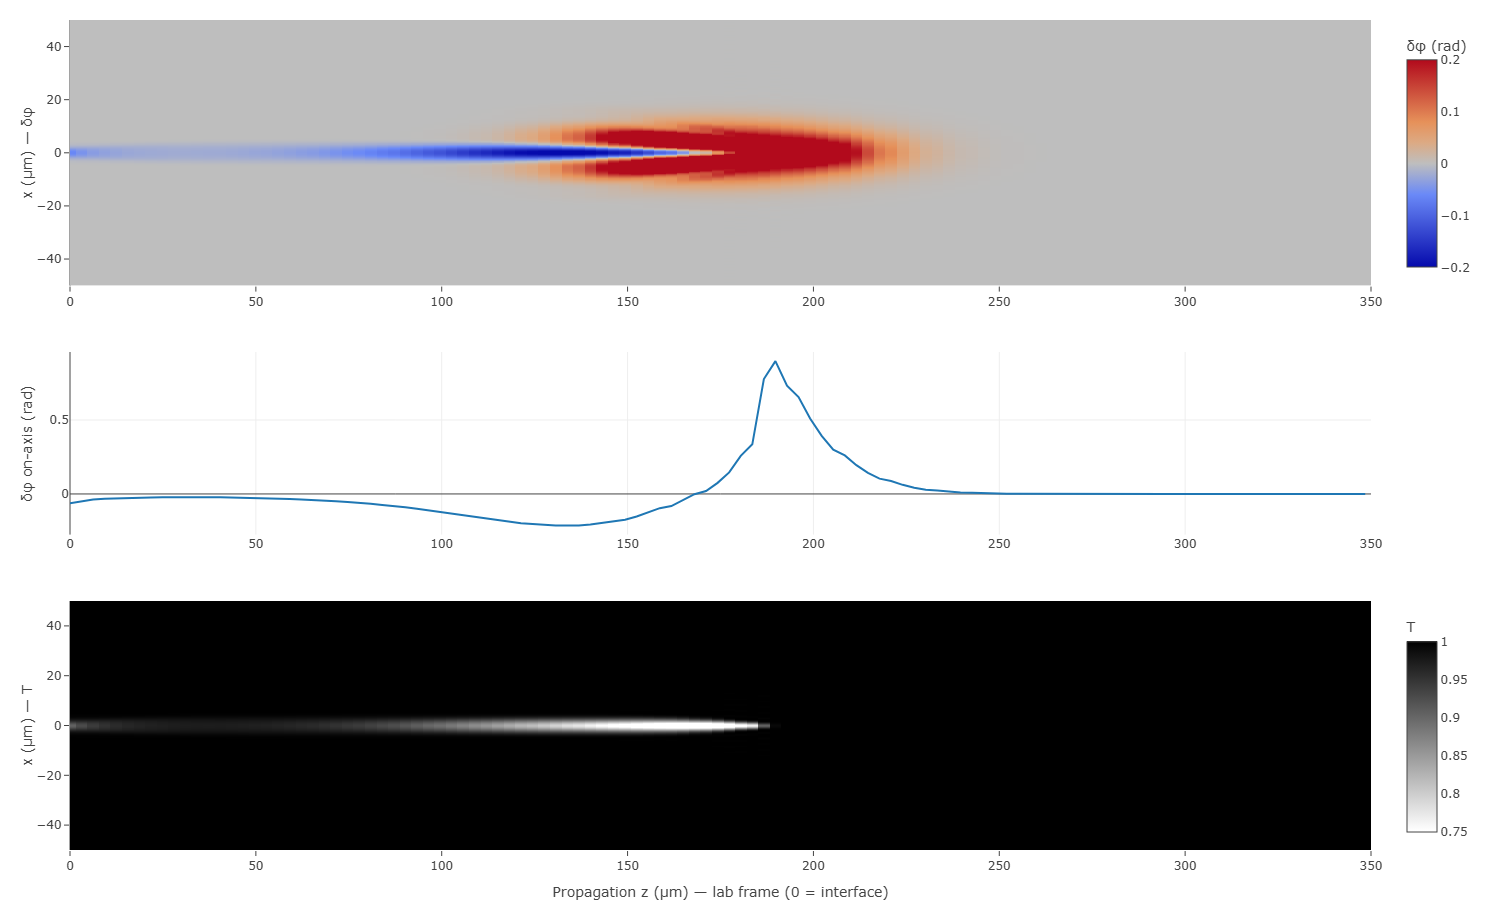
\includegraphics[width=\linewidth]{fig_probe_maps.png}
    \caption{What the diagnostic page shows for the $4\ \mu$J run at one probe delay. Top, the phase map $\delta\varphi(z,x)$ after the forward Abel transform and the numerical aperture filter, with the three $\Delta n$ channels summed. Middle, the same phase read along the axis. Bottom, the transmittance over the same plane, obtained from the imaginary part of the same permittivity. The phase is negative before the nonlinear focus, where free electrons dominate, and turns strongly positive around $z\simeq190\ \mu$m where the Kerr and trapped exciton contributions take over. The transmittance dips only along the thin channel where the electron density is high, which is the absorption counterpart of the negative phase region above it.}
    \label{fig:probe_maps}
\end{figure}

\begin{figure}[htbp]
    \centering
    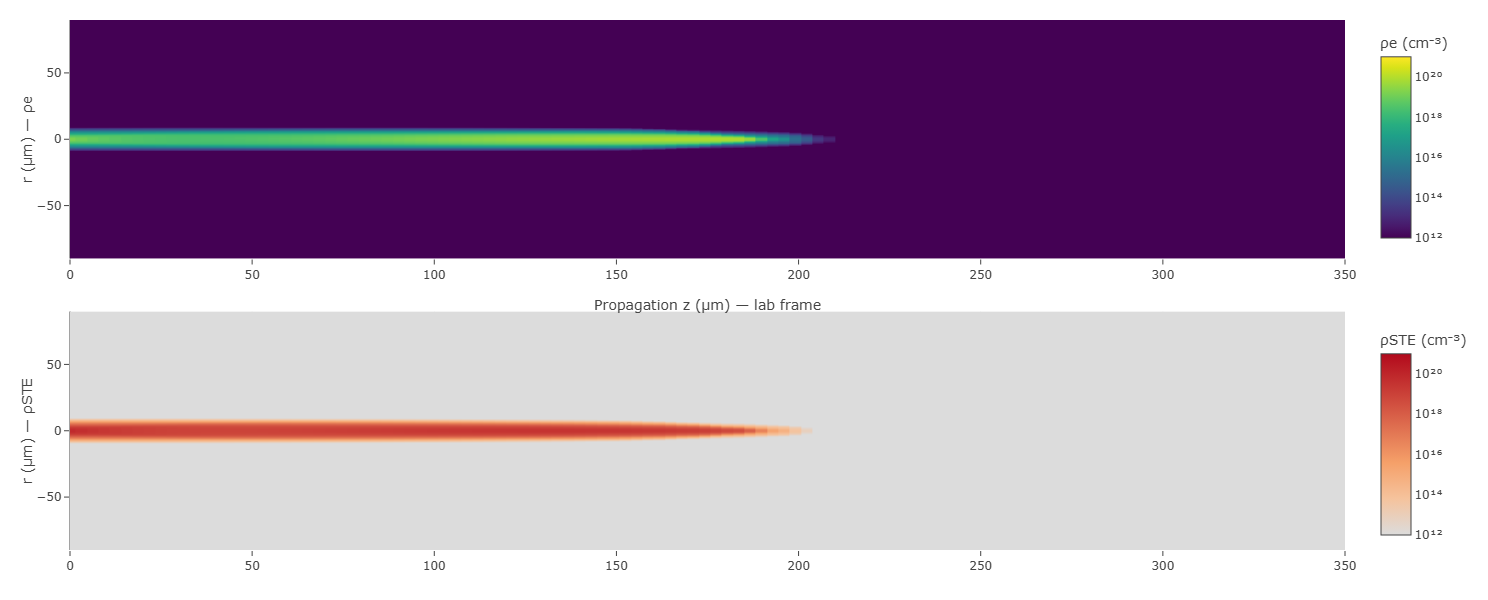
\includegraphics[width=\linewidth]{fig_probe_densities.png}
    \caption{Free electron density (top) and self-trapped exciton density (bottom) at the same delay as Figure~\ref{fig:probe_maps}, on a logarithmic scale. These are the densities the solver computed. They are shown because they explain the phase maps above.}
    \label{fig:probe_densities}
\end{figure}

\begin{figure}[htbp]
    \centering
    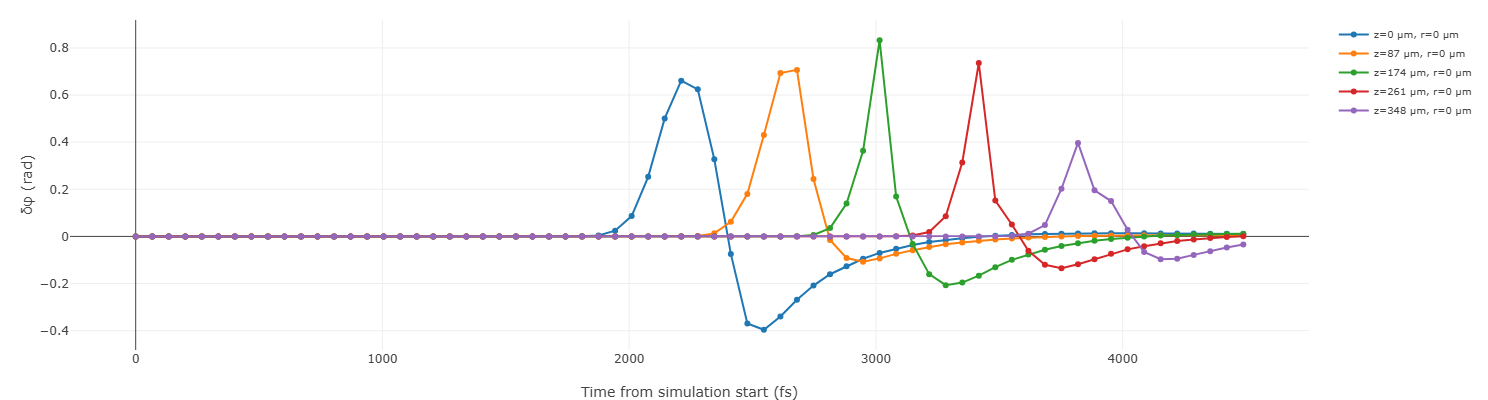
\includegraphics[width=\linewidth]{fig_dephasage_vs_z.png}
    \caption{On-axis probe phase shift as a function of time, at five planes along the propagation. Each curve shows the same three stage sequence, a positive peak while the pump is present, a swing to negative once free electrons appear, then a slow recovery toward zero as trapping and decay drain the population. The five peaks are staggered in time because the pump needs about $1.7\ \text{ps}$ to cross the $350\ \mu$m box, so a plane further along is reached later.}
    \label{fig:dephasage_vs_z}
\end{figure}
